\addcontentsline{toc}{chapter}{Занятие 4. Геометрические вероятности. Принцип отражения}
\chapter*{Занятие 4. Геометрические вероятности. Принцип отражения}

\addcontentsline{toc}{section}{Контрольные вопросы и задания}
\section*{Контрольные вопросы и задания}

\subsubsection*{Запишите формулу для вычисления геометрической вероятности.}

Случайным образом выбираются точки в области $D$, где:
$D \subset \mathbb{R}^n,
\Omega = \\
= D,
A \subset D$
--- случайное событие.
$$P \left( A \right) =
\frac{|A|}{| \Omega |}, $$
где $|A|$ --- $n$-мерный объём $A$.

Геометрическое определение вероятности обобщает классическое на случай бесконечного множества элементарных исходов
$ \Omega $ тогда, когда $ \Omega $ представляет собой подмножество пространства $ \mathbb{R}$ (числовой прямой),
$ \mathbb{R}^2$ (плоскости), $ \mathbb{R}^n$ ($n$-мерного евклидова пространства).

Под мерой $ \mu \left( A \right) $ подмножества $A$ будем понимать его длину,
площадь или объём (обобщённый объём) в зависимости от того,
какому пространству принадлежит $ \Omega $:
в  $ \mathbb{R}$, в $ \mathbb{R}^2$ или в $ \mathbb{R}^3 \left(  \mathbb{R}^n \right) $.

Вероятностью события $A$
называют число $P \left( A \right) $, равное отношению меры множества $A$ к мере множества $ \Omega $:
$$P \left( A \right) =
\frac{ \mu \left( A \right) }{ \mu \left( \Omega \right) },$$
где $ \mu \left( A \right) $ --- мера множества $A$.

\subsubsection*{В чём состоит принцип отражения?}

Пусть $A$ и $B$ --- точки с целыми координатами, причём $B$ лежит выше оси абсцисс и правее оси ординат, $B'$ --- точка, симметричная $B$ относительно оси абсцисс.

Количество путей, начинающихся в точке $A$ и оканчивающихся в точке $B$, которые касаются оси абсцисс или пересекают её, равно числу путей, оканчивающихся в точке $B'$.

\subsubsection*{Опишите математические модели вероятностного эксперимента, связанные с задачей про встречу и иглой Бюффона.}

\paragraph*{Задача о встрече}

\textit{Задание.} Два приятеля договорились встретиться на протяжении определённого времени $T$.
Первый приятель может ждать другого не больше чем время $ \tau_1$, а второй ждёт первого только время $ \tau_2$.
Чему равна вероятность встречи приятелей, если каждый из них независимо от другого может прийти равновероятно в любой момент промежутка времени $T$.

\textit{Решение.} Обозначим моменты прихода первого и второго приятелей через $x$ и $y$ соответственно.
Тогда пространство элементарных событий $ \Omega $ имеет вид (рис. \ref{fig:41}): $ \Omega = \left\{ \left( x, y \right): 0 \leq  x \leq T, 0 \leq y \leq T \right\} $.

\begin{figure}[h!]
  \centering
  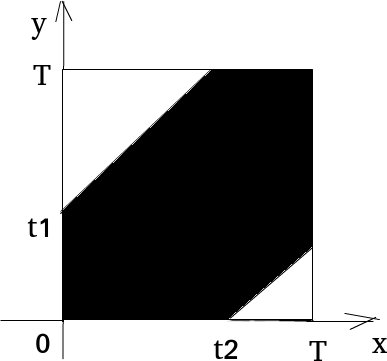
\includegraphics[width=.4\textwidth]{./pictures/4_1.png}
  \caption{Пространство элементарных событий}
  \label{fig:41}
\end{figure}

Множество $A$ точек, которые способствуют встрече, определяется неравенствами
$$A =
\left\{ \left( x, y \right):
0 \leq x \leq y \leq \min \left( T, x + \tau_1 \right),
0 \leq x \leq y \leq \min \left( T, x + \tau_2 \right) \right\}.$$

Очевидно, что
$$m \left( \Omega \right) =
T^2,
m \left( A \right) =
T^2 - \frac{1}{2} \left[ T - \min \left( T, \tau_1 \right) \right]^2 - \frac{1}{2} \left[ T - \min \left( T, \tau_2 \right) \right]^2.$$

Поэтому согласно с
$$P \left\{ A \right\} =
\frac{ \mu \left( A \right) }{ \mu \left( \Omega \right) }$$
имеем
$$P \left\{ A \right\} =
1 - \frac{1}{2} \left\{ \left[ \max \left( 0, 1 - \frac{ \tau_1}{T} \right) \right]^2 + \left[ \max \left( 0, 1 - \frac{ \tau_2}{T} \right) \right]^2 \right\}.$$

\paragraph*{Игла Бюффона}

\textit{Задание.} Рассмотрим плоскость, разделённую параллельными прямыми, которые находятся на расстоянии $2a$ одна от другой (рис. \ref{fig:42}).
На плоскость наугад бросается игла, которая имеет длину $2l$.
Нужно найти вероятность того, что игла пресечёт хотя бы одну из прямых (в случае $l > a$ игла может пересечь несколько прямых).

\begin{figure}[h!]
  \centering
  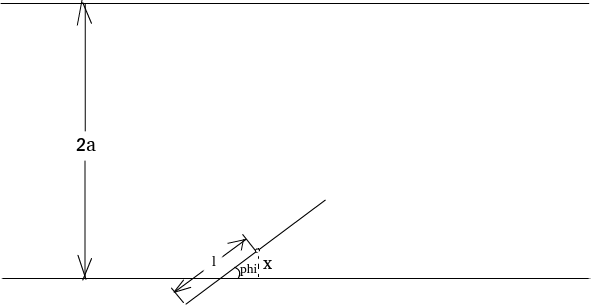
\includegraphics[width=.9\textwidth]{./pictures/4_2.png}
  \caption{Плоскость, разделённая параллельными прямыми}
  \label{fig:42}
\end{figure}

\textit{Решение.}  Положение иглы однозначно определяется расстоянием от центра игла до ближайшей прямой и углом $ \phi $, который образует игла с этой прямой.
Очевидно, что $0 \leq x \leq a$ и $0 \leq \phi \leq \pi $, т.е. пространство элементарных событий $ \Omega $ является прямоугольником (рис. \ref{fig:4201} и \ref{fig:4202}):
$$ \Omega =
\left\{ \left( x, \phi \right):
0 \leq x \leq a,
0 \leq \phi \leq \pi \right\}.$$

Для того, чтобы игла пересекла одну из прямых необходимо и достаточно выполнение условия
$x \leq l \sin \phi$, т.е.
$$A =
\left\{ \left( x, \phi \right):
x \leq l \sin \phi,
0 \leq x \leq a,
0 \leq \phi \leq \pi \right\}.$$

Рассмотрим два случая.

А. $l \leq a$ (рис. \ref{fig:4201}).
Очевидно, что
$$ \mu \left( \Omega \right) =
a \pi,
\mu \left( A \right) =
\int \limits_{0}^{ \pi } l \sin \phi d \phi =
2l,
P \left\{ A \right\} =
\frac{2l}{a \pi}.$$

B. $l > a$ (рис. \ref{fig:4202}).
В этом случае имеем
\begin{equation*}
\begin{split}
\mu \left( A \right) =
a \pi - 2 \int \limits_{0}^{\arcsin \left( \frac{a}{l} \right) } \left( a - l \sin \phi \right) d \phi =
a \left( \pi - 2 \arcsin \frac{a}{l} \right) + \\
+ 2l \left( 1 - \sqrt{1 - \left( \frac{a}{l} \right)^2} \right),
P \left\{ A \right\} =
\frac{ \mu \left( A \right) }{a \pi}.
\end{split}
\end{equation*}

\begin{figure}[h!]
  \centering
  \begin{minipage}[b]{0.4\textwidth}
    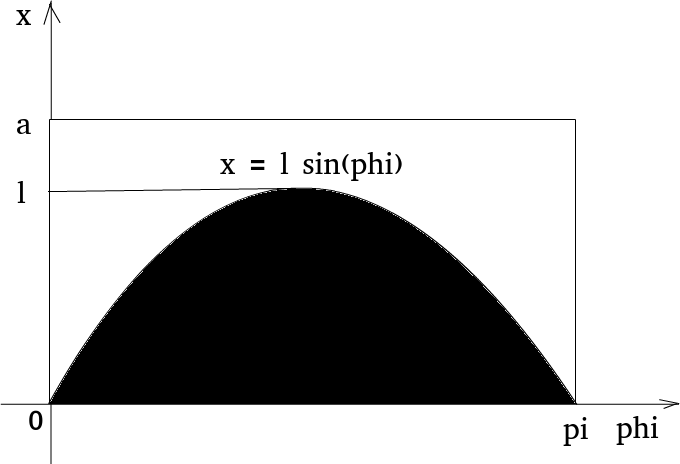
\includegraphics[width=\textwidth]{./pictures/4_201.png}
    \caption{Случай $l \leq a$}
    \label{fig:4201}
  \end{minipage}
  \hfill
  \begin{minipage}[b]{0.4\textwidth}
    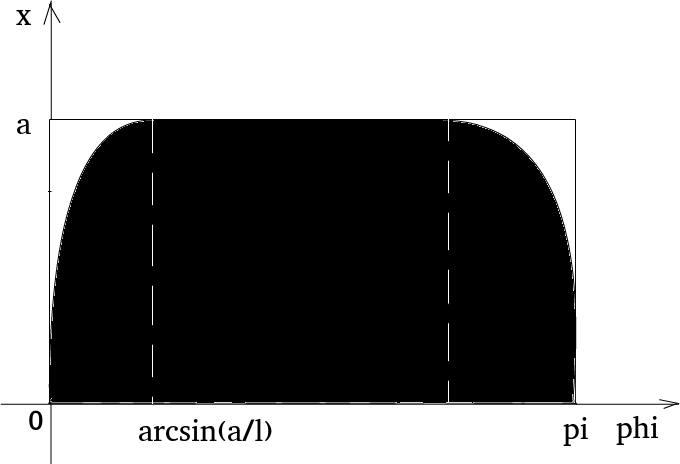
\includegraphics[width=\textwidth]{./pictures/4_202.png}
    \caption{Случай $l > a$}
    \label{fig:4202}
  \end{minipage}
\end{figure}

В случае $l \leq a$ с помощью иглы Бюффона можно приближённо вычислить число $ \pi $.
Действительно, пусть было проведено $n$ экспериментов, в каждом из которых исследовалось пересекла ил игла прямую, или нет.
Обозначим через $ \nu_n$ количество экспериментов, в которых произошло пересечение.
Согласно с усиленным законом больших чисел
$$ \frac{ \nu_n}{n} \xrightarrow[n \rightarrow \infty ]{} P \left\{ A \right\} =
\frac{2l}{a \pi}$$
с вероятностью 1.

Отсюда следует, что
$$ \frac{2l n}{a \nu_n} \xrightarrow[n \rightarrow \infty ]{} \pi $$
с вероятностью 1, т.е. с помощью достаточного количества экспериментов можно вычислить число $ \pi $ с любой точностью.

\addcontentsline{toc}{section}{Аудиторные задачи}
\section*{Аудиторные задачи}

\subsubsection*{4.3}

\textit{Задание.} На отрезке $ \left[ 0, 10 \right] $ числовой оси наугад выбрана точка.
Найдите вероятность того, что расстояние от этой точки до средины отрезка окажется большим чем три.

\textit{Решение.} Обозначим через $x$ расстояние от начала отрезка к точке.
Тогда пространством элементарных событий является отрезок
$ \Omega = \\
= \left\{ x \in \mathbb{R}: \, 0 \leq x \leq 10 \right\} =
\left[ 0, 10 \right] $,
а событию $A$ =
\{расстояние от точки до средины отрезка окажется большим чем 3\}
способствуют точки объединения интервала
$A =
\left\{ x \in \Omega: \, x < 2, \, x > 8 \right\} =
\left[0, 2 \right) \cup \left(8, 10 \right] $.
Поэтому
$$P \left( A \right) =
\frac{|A|}{| \Omega |} =
\frac{4}{10} =
\frac{2}{5}.$$

\subsubsection*{4.4}

\textit{Задание.} В квадрате $ABCD$ со стороной 3 наугад выбрана точка.
Найдите вероятность того, что расстояние от этой точки к:
\begin{enumerate}[label=\alph*)]
\item центру квадрата;
\item стороне $AB$;
\item точке $A$;
\item одной из сторон;
\item диагонали $AC$ не будет превышать 1.
\end{enumerate}

\textit{Решение.} Обозначим через $x$ и $y$ координаты точки.
Пусть точка $A$ имеет координаты $ \left( 0, 0 \right) $,
точка $B$ --- $ \left( 0, 3 \right) $, $C$ --- $ \left( 3, 3 \right) $, и $D$ имеет координаты $ \left( 3, 0 \right) $.
Тогда пространством элементарных событий является квадрат
$ \Omega = \\
=\left\{ \left( x, y \right) \in \mathbb{R}^2: \,
0 \leq x \leq 3,
0 \leq y \leq 3 \right\} $.
Площадь квадрата равна $S_{\Omega} = 3^2 = \\ = 9$.

\begin{enumerate}[label=\alph*)]
\item Центр квадрата --- это точка $ O \left( 3/2, 3/2 \right) $.
Расстояние от точки к центру квадрата не должно превышать единицу --- событие $A$.
Тогда точка должна находиться в круге с радиусом 1 и центром в точке $O$.
Событие описывается множеством
$$A =
\left\{ \left( x, y \right) \in \Omega: \,
\left( \frac{3}{2} - x \right)^2 + \left( \frac{3}{2} - y \right)^2 \leq 1 \right\}.$$

Поэтому
$$P \left( A \right) =
\frac{S_A}{S_{ \Omega }} =
\frac{ \pi \cdot 1^2}{9} =
\frac{ \pi }{9};$$

\item событие $A$ =
\{расстояние от точки к стороне $AB$ не будет превышать единицу\}
описывается множеством $A = \left\{ \left( x, y \right) \in \Omega: \, 0 \leq x \leq 1, 0 \leq y \leq 3 \right\} $.
Изобразив $A$ на плоскости, можно убедиться, что точки множества $A$ образуют прямоугольник со сторонами $1$ и $3$.
Поэтому
$$P \left( A \right) =
\frac{S_A}{S_{ \Omega }} =
\frac{1 \cdot 3}{9} =
\frac{1}{3};$$

\item событие $A =$
\{расстояние к точке $A$ не будет превышать единицу\}
описывается множеством $A =\left\{ \left( x, y \right) \in \Omega: \, x^2 + y^2 \leq 1 \right\} $.
Изобразив $A$ на плоскости, можно убедиться, что $A$ является четвертью круга с центром в начале координат и радиусом 1.
Поэтому
$$P \left( A \right) =
\frac{S_A}{S_{ \Omega }}=
\frac{ \frac{1}{4} \cdot \pi 1^2}{9} =
\frac{ \pi }{36};$$

\item событие $A =$
\{расстояние от точки к одной из сторон не превышает единицу\}
описывается множеством
$$A =
\left\{ \left( x, y \right) \in \Omega: \,
0 \leq x \leq 1,
2 \leq x \leq 3,
0 \leq y \leq 1,
2 \leq y \leq 3 \right\}.$$
Изобразив $A$ на плоскости, можно убедиться, что $A$ --- исходный квадрат с вырезанным квадратом со стороной 1.
Поэтому
$$P \left( A \right) =
\frac{S_A}{S_{ \Omega }} =
\frac{3^2 - 1^2}{9} =
\frac{9-1}{9} =
\frac{8}{9};$$

\item событие $A =$
\{расстояние от точки к диагонали $AC$ не превысит единицы\}
описывается множеством $A = \left\{ \left( x, y \right) \in \Omega: \, 0 \leq \left| y - x \right| \leq 1 \right\}$.
Изобразив $A$ на плоскости, можно убедиться,
что $A$ является квадратом без двух прямоугольных равнобедренных треугольников с катетами $3 - \sqrt{2}$.
Поэтому
$$P \left( A \right) =
\frac{S_A}{S_{ \Omega }} =
\frac{3^2 - 2 \cdot \frac{1}{2} \cdot \left( 3 - \sqrt{2} \right)^2}{9} =
\frac{9 - \left( 3 - \sqrt{2} \right)^2}{9}.$$
\end{enumerate}

\subsubsection*{4.5}

\textit{Задание.} Точка $ \left( \xi, \eta \right) $ наугад выбрана в квадрате $ \left[ 0, 1 \right]^2$.
Для фиксированного $z \in \left( 0, 1 \right) $ вычислить вероятность:
\begin{enumerate}[label=\alph*)]
\item $P \left( \left| \xi - \eta \right| < z \right) $;
\item $P \left( \min \left( \xi, \eta \right) < z \right) $;
\item $P \left( \left( \xi + \eta \right)/2 < z \right) $.
\end{enumerate}

\textit{Решение.}
Пространство элементарных событий можно описать следующим образом:
$ \Omega =
\left\{ \left( \xi, \eta \right) \in \left[ 0, 1 \right]^2 \right\} $.
Изобразив $ \Omega $ на плоскости, можно убедиться, что $ \Omega $ является квадратом со стороной 1.

\begin{enumerate}[label=\alph*)]
\item Событие $A$ описывается множеством
$$A =
\left\{ \left( \xi, \eta \right) \in \Omega: \,
\left| \xi - \eta \right| < z,
z \in \left( 0, 1 \right) \right\}.$$
Изобразив $A$ на плоскости,
можно убедиться,
что точки множества $A$ образуют квадрат с двумя вырезанными прямоугольными равнобедренными треугольниками с катетами $1 - z$.

Найдём площадь треугольника:
$$S = \frac{1}{2} \cdot \left( 1-z \right)^2 =
\frac{ \left( 1-z \right)^2}{2}.$$

Тогда вероятность равна
$$P \left( A \right) =
1 - 2 \cdot \frac{ \left( 1-z \right)^2}{2} =
1 - \left( 1-z \right)^2 =
1 - 1 + 2z - z^2 =
z \left( 2-z \right);$$

\item событие
$A =
\left\{ P \left( \min \left( \xi, \eta \right) < z \right) \right\}$
описывается множеством
$A = \\
= \left\{ \left( \xi, \eta \right) \in \Omega: \,
\min \left( \xi, \eta \right) < z, \,
z \in \left( 0, 1 \right) \right\} $.
Изобразив $A$ на плоскости,
можно убедиться, что точки множества $A$ образуют квадрат со сторонами длиной $1$ без квадрата со стороной длиной $1 - z$ (рис. \ref{fig:45}, \ref{fig:451}).

\begin{figure}[h!]
  \centering
  \begin{minipage}[b]{0.4\textwidth}
    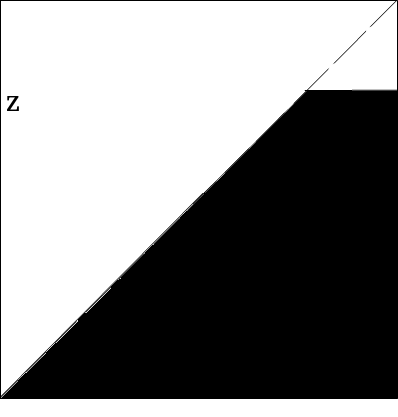
\includegraphics[width=\textwidth]{./pictures/4_5.png}
    \caption{$ \xi < \eta, \min \left( \xi, \eta \right) = \\ = \eta < z$}
    \label{fig:45}
  \end{minipage}
  \hfill
  \begin{minipage}[b]{0.4\textwidth}
    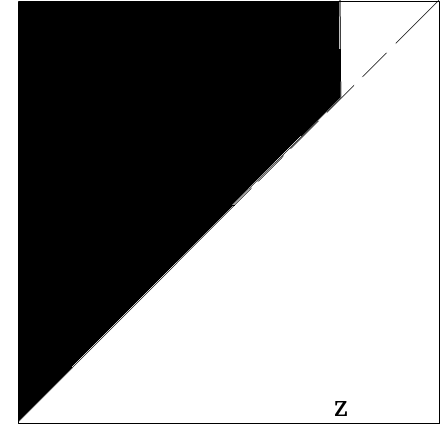
\includegraphics[width=\textwidth]{./pictures/4_5_1.png}
    \caption{$ \xi \geq \eta, \min \left( \xi, \eta \right) = \\ = \xi < z$}
    \label{fig:451}
  \end{minipage}
\end{figure}

Поэтому
$$P =
1 - \left( 1-z \right)^2;$$

\item рассмотрим случай, когда $2z < 1$.
Упростим неравенство. Умножим левую и правую части на $2$.
Получим: $ \xi + \eta < 2z$.
Выразим $ \xi $ и $ \eta: \, \xi < \\ < 2z - \eta, \, \eta < 2z - \xi $.

Событие
$$A =
\left\{ P \left( \frac{ \xi + \eta }{2} < z \right) \right\} $$
описывается множеством
$$A =
\left\{ \left( \xi, \eta \right) \in \Omega: \,
\frac{ \xi + \eta }{2} < z, \,
z \in \left( 0, 1 \right) \right\}.$$
Изобразив $A$ на плоскости, можно убедиться, что точки множества $A$ образуют прямоугольник с катетами $2z$ (рис. \ref{fig:452}).

\begin{figure}[h!]
  \centering
  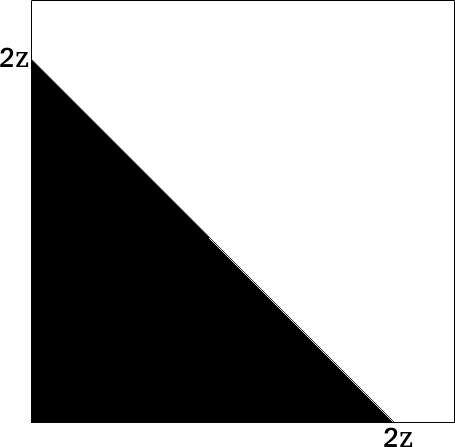
\includegraphics[width=.4\textwidth]{./pictures/4_5_2.png}
  \caption{Точки множества $A, \, 2z < 1$}
  \label{fig:452}
\end{figure}

Поэтому
$$P \left( A \right) =
\frac{S_A}{S_{ \Omega }} =
\frac{ \frac{1}{2} \cdot 2z \cdot 2z}{1 \cdot 1} =
2z^2.$$
\end{enumerate}

Теперь рассмотрим случай, когда $2z > 1$ (рис. \ref{fig:453}).

\begin{figure}[h!]
  \centering
  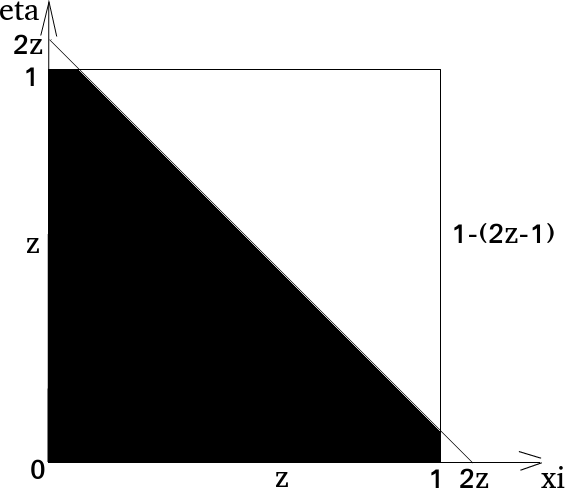
\includegraphics[width=.4\textwidth]{./pictures/4_5_3.png}
  \caption{Точки множества $A, \, 2z > 1$}
  \label{fig:453}
\end{figure}

Вероятность тогда равна
$$P \left( A \right) =
1 - \frac{1}{2} \cdot \left( 2-2z \right)^2 =
1 - 2 \left( 1-z \right)^2.$$

\subsubsection*{4.6}

\textit{Задание.} На отрезке $ \left[ 0, 10 \right] $ числовой оси наугад выбраны две точки.
Найдите вероятность того, что расстояние от правой точки к точке с координатой $8$ окажется меньшим чем единица.

\textit{Решение.} Обозначим через $x$ и $y$ расстояния от начала отрезка (точки $0$) к левой и правой точкам соответственно.
Тогда пространство элементарных событий можно описать следующим образом:
$$ \Omega =
\left\{ \left( x, y \right) \in \mathbb{R}^2: \,
0 \leq x  \leq y \leq 10 \right\},$$
а событие $A =$
\{расстояние от правой точки к точке 8\} описывается множеством $A = \left\{ \left( x, y \right) \in \Omega: \left| \max \left( x, y \right) - 8 \right| < 1 \right\} $.
Изобразив $ \Omega $ и $A$ на плоскости, можно убедиться, что $ \Omega $ является фигурой, изображённой на рис. \ref{fig:46}.

\begin{figure}[h!]
  \centering
  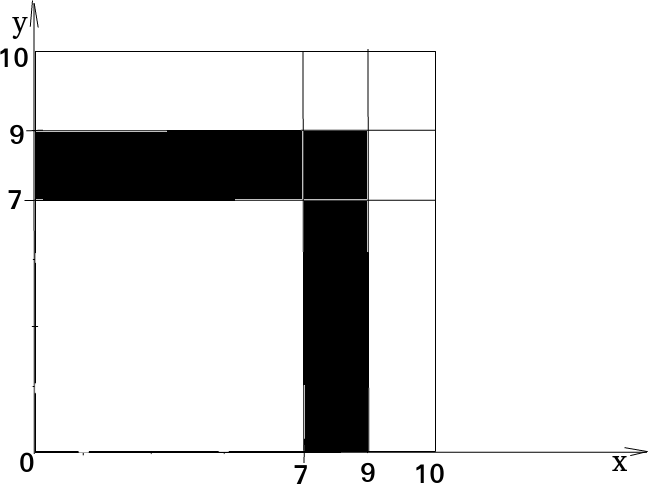
\includegraphics[width=.4\textwidth]{./pictures/4_6.png}
  \caption{Точки множества $A$}
  \label{fig:46}
\end{figure}

Поэтому
$$P \left( A \right) =
\frac{S_A}{S_{ \Omega }} =
\frac{9^2-7^2}{10 \cdot 10} =
\frac{2 \cdot 16}{100} =
\frac{32}{100} =
0.32.$$

\subsubsection*{4.7}

\textit{Задание.} На отрезке $AB$ длиной $a$ наугад выбраны, независимо одна от другой, шесть точек.
Найдите вероятность того, что:
\begin{enumerate}[label=\alph*)]
\item две точки будут находиться от точки $A$ на расстоянии, меньшем чем $b$, а четыре точки --- на расстоянии, большем чем $b \, \left(b<a \right) $;
\item две точки будут находиться от точки $A$ на расстоянии, меньшем чем $c$, одна --- на расстоянии, не меньшем чем $c$ и не большем чем $b$,
и три точки --- на расстоянии, большем чем $b \, \left( c<b<a \right) $.
\end{enumerate}

\textit{Решение.} Обозначим через $x_1, \, x_2, \dotsc, x_6$ расстояния от точки $A$ к выбранным точкам.
Элементарный исход ---  кортеж расстояний от точки $A: \, \omega = <x_1, \, x_2, \dotsc, x_6>$.
Тогда пространство элементарных исходов можно описать следующим образом:
$$ \Omega =
\left\{ <x_1, \, x_2, \dotsc, x_6> \in AB^6:
0 \leq x_1 \leq a, \,
0 \leq x_2 \leq a, \dotsc,
0 \leq x_6 \leq a \right\}.$$

\begin{enumerate}[label=\alph*)]
\item Событие $A =$
\{две точки будут находиться от точки $A$ на расстоянии,
меньшем чем $b$, а четыре точки --- на расстоянии,
большем чем $b \, \left( b<a \right) $\}
описывается множеством
\begin{equation*}
\begin{split}
A = \\
\left\{ <x_1, x_2, \dotsc, x_6> \in \Omega: \,
0 \leq x_1 < b, \,
0 \leq x_2 < b, \,
b < x_3 \leq a, \dotsc,
b < x_6 \leq a \right\}.
\end{split}
\end{equation*}
Возьмём нормированное расстояние $x_i/AB$, чтобы все точки были из $ \left[ 0, 1 \right] $.
Потому $b$ теперь $b/a$.
Событие $A$ примет вид:
$$A =
\left\{ <x_1, \, x_2, \dotsc, x_6> \in \Omega:
x_1 < \frac{b}{a}, \,
x_2 < \frac{b}{a}, \,
x_3 > \frac{b}{a}, \,
x_4 > \frac{b}{a}, \,
x_5 > \frac{b}{a}, \,
x_6 > \frac{b}{a} \right\}.$$

Изобразим двумерный случай (рис. \ref{fig:47}).

\begin{figure}[h!]
  \centering
  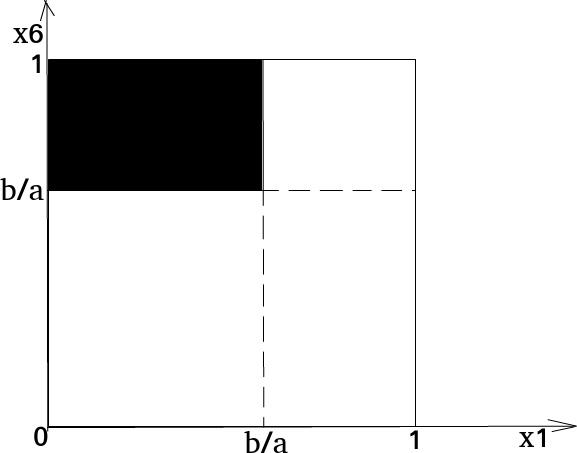
\includegraphics[width=.4\textwidth]{./pictures/4_7.png}
  \caption{Двумерный случай ($x_1$ и $x_6$)}
  \label{fig:47}
\end{figure}

Теперь трёхмерные случаи ($x_1, \, x_2, \, x_6$ и $x_1, \, x_5, \, x_6$) --- рис. \ref{fig:471}.

\begin{figure}[h!]
  \centering
  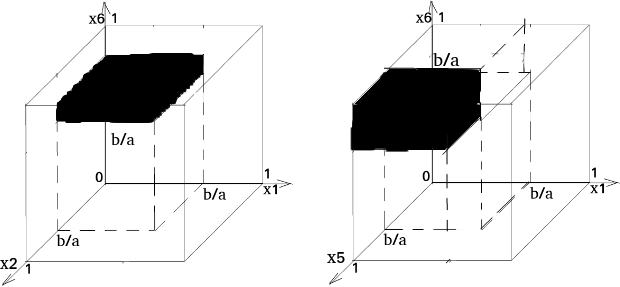
\includegraphics[width=.7\textwidth]{./pictures/4_7_1.png}
  \caption{Трёхмерные случаи}
  \label{fig:471}
\end{figure}

Это параллелепипед со сторонами длиной $b/a$ и $1 - b/a$.
Для 6-мерного случая, его мера равна
$$ \left( \frac{b}{a} \right)^2 \left( 1 - \frac{b}{a} \right)^4.$$
Осталось учесть перестановки, ведь нет разницы, какая точка будет слева: первая или пятая.
Нужно выбрать две точки из шести, которые будут слева от $b/a$.
Посчитали 1 случай, а таких случаев $C_6^2$.
Тогда вероятность равна
$$P =
\frac{C_6^2 \left( \frac{b}{a} \right)^2 \left( 1 - \frac{b}{a} \right)^4}{1^6} =
15 \left( \frac{b}{a} \right)^2 \left( 1 - \frac{b}{a} \right)^4;$$

\item событие $A =$
\{две точки будут находиться от точки $A$ на расстоянии,
меньшем чем $c$ и не большем чем $b$, и три точки ---
на расстоянии, большем чем
$b \,
\left( c<b<a \right)$
описывается множеством
\begin{equation*}
\begin{split}
A = \\
\left\{ <x_1, \, x_2, \dotsc, x_6> \in \Omega: \,
_1 < c, \,
x_2 < c, \,
c \leq x_3 \leq b, \,
b < x_4, \,
b < x_5, \,
b < x_6 \right\}.
\end{split}
\end{equation*}

Возьмём нормированное расстояние $x_i/AB$, чтобы все они были из $ \left[ 0, 1 \right] $.
Потому теперь
\begin{equation*}
\begin{split}
A = \\
\left\{ <x_1, \dotsc, x_6> \in \Omega:
x_1 < \frac{c}{a},
x_2 < \frac{c}{a},
\frac{c}{a} \leq x_3 \leq \frac{b}{a},
\frac{b}{a} < x_4,
\frac{b}{a} < x_5,
\frac{b}{a} < x_6 \right\}.
\end{split}
\end{equation*}

Для 6-мерного случая мера этой фигуры равна
$$ \left( \frac{c}{a} \right)^2 \left( \frac{b}{a} - \frac{c}{a} \right) \left( 1 - \frac{b}{a} \right)^3.$$

Осталось учесть перестановки, ведь нет разницы, какая точка где будет находиться.
Нужно выбрать две точки из шести, которые будут находиться слева от $c/a$ --- это $C_6^2$, а затем одну точку из четырёх, которая будет между $c/a$ и $b/a$ --- $C_4^1$.
Тогда вероятность равна
$$P =
C_6^2 C_4^1 \left( \frac{c}{a} \right)^2 \left( \frac{b}{a} - \frac{c}{a} \right) \left( 1 - \frac{b}{a} \right)^3.$$
\end{enumerate}

\subsubsection*{4.8}

\textit{Задание.} Точку $ \left( \xi, \eta \right) $ выбрано в квадрате $ \left[ 0, 1 \right]^2$.
Найдите вероятность того, что уравнение $x^2 + \xi x + \eta = 0$ имеет:
\begin{enumerate}[label=\alph*)]
\item действительные разные корни;
\item кратные корни.
\end{enumerate}

\textit{Решение.}
Пространство элементарных событий можно описать следующим образом:
$ \Omega =
\left\{ \left( \xi, \eta \right) \in \left[ 0, 1 \right]^2 \right\} $.
Найдём дискриминант квадратного уравнения: $D = \xi^2 - 4 \eta $.

\begin{enumerate}[label=\alph*)]
\item Чтобы уравнение имело 2 разных действительных корня, его дискриминант должен быть больше нуля: $ \xi^2 - 4 \eta > 0$ или $ \xi^2 > 4 \eta $.
Выразив $ \eta $, получим:
$$ \eta < \frac{ \xi^2}{4}.$$
На рисунке \ref{fig:48} эта область изображена голубым цветом.

\begin{figure}[h!]
  \centering
  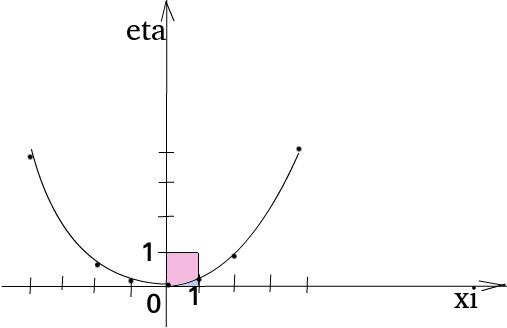
\includegraphics[width=.7\textwidth]{./pictures/4_8.png}
  \caption{$ \eta = \frac{ \xi^2}{4}$}
  \label{fig:48}
\end{figure}

Найдём площадь под кривой:
$$S =
\int \limits_0^1 \frac{ \xi^2}{4}d \xi =
\left. \frac{ \xi^3}{12} \right|_0^1 =
\frac{1}{12}.$$

Тогда вероятность равна
$$P =
\frac{ \frac{1}{12} }{1 \cdot 1} =
\frac{1}{12}.$$

\item чтобы уравнение имело кратные корни, его дискриминант должен быть равен нулю --- эта облась обозначена линией на рисунке.
Плозадь линии равна нулю, поэтому вероятность данного события тоже равна нулю.
\end{enumerate}

\subsubsection*{4.9}

\textit{Задание.} На окружности наугад выбраны три точки $A, \, B$ и $C$.
Найдите вероятность того, что треугольник $ABC$ окажется:
\begin{enumerate}[label=\alph*)]
\item остроугольным;
\item прямоугольным.
\end{enumerate}

\textit{Решение.} Окружность симметрична, поэтому можем выбрать начало отсчёта в точке $A$.
Обозначим через $x$ и $y$ длины дуг от начала отсчёта к точкам $B$ и $C$.
Тогда пространство элементарных событий можно описать следующим образом:
$ \Omega =
\left\{ \left( x, y \right) \in \left[0, 2 \pi \right]^2 \right\}$.
Изобразив $ \Omega $ на плоскости, можно убедиться, что $ \Omega $ является квадратом со стороной $2 \pi$.
Поэтому $S_{ \Omega } = 2 \pi \cdot 2 \pi = 4 \pi^2$.

\begin{enumerate}[label=\alph*)]
\item Событие $A =$
\{треугольник $ABC$ окажется остроугольным\}
описывается множеством
$A =
\left\{ \left( x, y \right) \in \left[ \pi, 2 \pi \right]^2 \right\}$,
т.к. вершины остроугольного треугольника должны находиться по разные стороны от диаметра окружности.
Изобразив $A$ на плоскости, можно убедиться, что точки множества $A$ образуют квадрат со сторонами длиной $ \pi $.
Поэтому $S_A = \pi \cdot \pi = \pi^2$.

Тогда вероятность события $A$ равна
$$P \left( A \right) =
\frac{S_A}{S_{ \Omega }} =
\frac{ \pi^2}{4 \pi^2} =
\frac{1}{4};$$
\item рассмотрим событие $A =$ \{треугольник $ABC$ окажется прямоугольным\}.
Оно описывается множеством
$$A = \left\{ \left( x, y \right) \in \Omega: \, y - x = \pi, x - y = \pi \right\}.$$	
Изобразив $A$ на плоскости, можно убедиться, что точки множества $A$ образуют прямые.
Площадь прямой равна нулю.
Поэтому вероятность события $A$ равна
$P \left( A \right) =
\frac{S_A}{S_{ \Omega }} =
\frac{0}{4 \pi^2} =
0.$
\end{enumerate}

\subsubsection*{4.10}

\textit{Задание.} Две лодки должны подойти к одному причалу.
Появление лодок --- независимые случайные события, равновероятные на протяжении суток.
Найдите вероятность того,
что ни одной из лодок де придётся ждать освобождения причала, если стоянка первой лодки --- один час, а второй --- два часа.

\textit{Решение.} Найдём вероятность того, что лодки <<встретятся>>.
Обозначим моменты появления первой и второй лодок через $x$ и $y$.
Тогда пространство элементарных событий $ \Omega $ имеет вид
(рис. \ref{fig:410}):
$$ \Omega = \left\{ \left( x, y \right): \, 0 \leq x \leq 24, \, 0 \leq y \leq 24 \right\}.$$

\begin{figure}[h!]
  \centering
  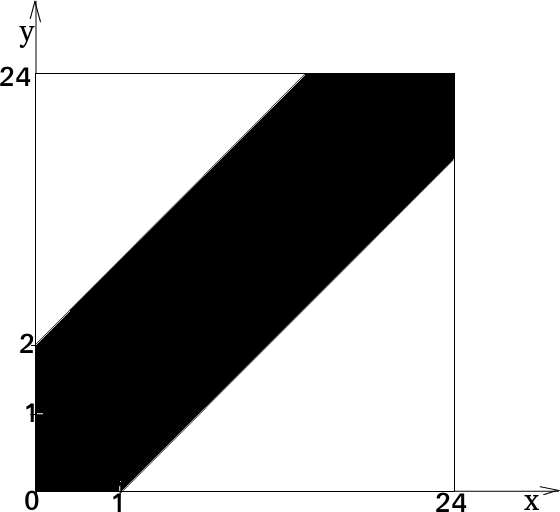
\includegraphics[width=.7\textwidth]{./pictures/4_10.png}
  \caption{Пространство элементарных событий}
  \label{fig:410}
\end{figure}

Множество $A$ точек, которые способствуют встрече, определяется неравенствами
$$A =
\left\{ \left( x, y \right) \in \Omega: \,
0 \leq x \leq y \leq \min \left( 24, x+1 \right), \,
0 \leq x \leq y \leq \min \left( 24, x+2 \right) \right\}.$$

Очевидно, что
\begin{equation*}
\begin{split}
 \mu \left( \Omega \right) = 24^2,
\mu \left( A \right) =
24^2 - \frac{1}{2} \left[ 24 - \min \left( 24, 1 \right) \right]^2 - \frac{1}{2} \left[ 24 - \min \left( 24, 2 \right) \right]^2 = \\
= 24^2 - \frac{1}{2} \left[ 24 - 1 \right]^2 - \frac{1}{2} \left[ 24 - 2 \right]^2 =
24^2 - \frac{1}{2} \cdot 23^2 - \frac{1}{2} \cdot 22^2.
\end{split}
\end{equation*}

Поэтому согласно с
$$P \left\{ A \right\} =
\frac{ \mu \left( A \right) }{ \mu \left( \Omega \right) }$$
имеем
$$P \left\{ A \right\} =
\frac{24^2 - \frac{1}{2} \cdot 23^2 - \frac{1}{2} \cdot 22^2}{24^2} =
1 - \frac{1}{2 \cdot 24^2} \left\{ 23^2 + 22^2 \right\}.$$

Тогда вероятность того, что лодки не <<встретятся>> равна вероятность противоположного события, т.е.
\begin{equation*}
\begin{split}
P \left\{ \overline{A} \right\} =
1 - \left( 1 - \frac{1}{2 \cdot 24^2} \left\{ 23^2 + 22^2 \right\} \right) =
1 - 1 + \frac{1}{2 \cdot 24^2} \left\{ 23^2 + 22^2 \right\} = \\
= \frac{1}{2 \cdot 24^2} \left\{ 23^2 + 22^2 \right\}.
\end{split}
\end{equation*}

\subsubsection*{4.11}

\textit{Задание.}
Путём $ \left\{ S_1, \dotsc, S_x \right\} $
из начала координат в точку
$ \left( x, y \right), \,
x \in \mathbb{N}, \,
y \in \mathbb{Z}$
называется ломаная с вершинами в точках
$ \left( 0, 0 \right), \, \left( 1, S_1 \right), \dotsc, \left( x, S_x \right) $, где $S_x = y, \, S_i - S_{i-1} \in \left\{ -1, 1 \right\} $.
Подсчитайте количество путей:
\begin{enumerate}[label=\alph*)]
\item из $ \left( 0, 0 \right) $ в $ \left( x, y \right) $;
\item из $ \left( 0, 0 \right) $ в $ \left( x, y \right) $, при условии, что $S_1 > 0, \dotsc, S_{x-1} > 0, \, S_x = y > 0$;
\item из $ \left( a, b \right) $ в $ \left( x, y \right) $, которые не пересекают ось абсцисс, при условии, что $a < x, \, x > 0, \, y > 0$.
\end{enumerate}

\textit{Решение.}

\begin{enumerate}[label=\alph*)]
\item Задача изображена на рисунке \ref{fig:411}.

\begin{figure}[h!]
  \centering
  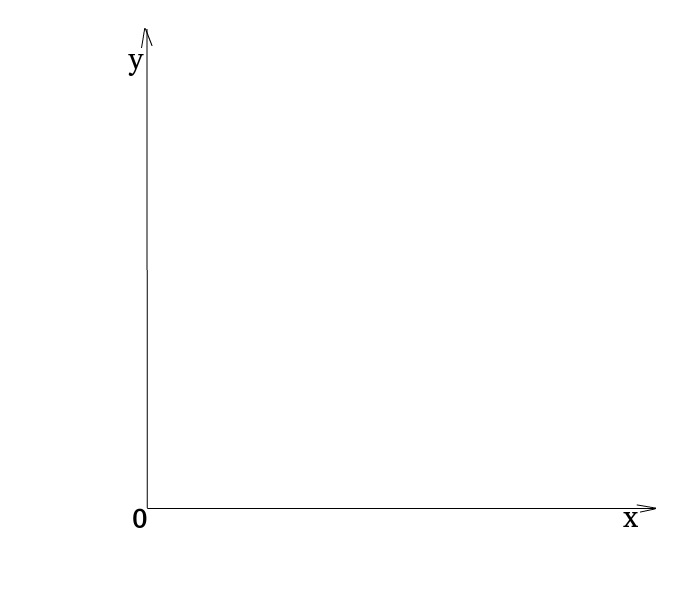
\includegraphics[width=.7\textwidth]{./pictures/4_11.png}
  \caption{Пути из точки $ \left( 0, 0 \right) $ к точке $ \left( x, y \right) $}
  \label{fig:411}
\end{figure}

Переворачиваем изображение --- получаем прямоугольник со сторонами $x'$ и $y'$.
В задании 4.22 уже нашли стороны полученного прямоугольника.
Они равны
$$x' = \frac{x+y}{2}, \, y' = \frac{x-y}{2}.$$

Нужно выбрать шаги, на которых будем перемещаться вверх, тогда на всех остальных шагах остаётся переместиться вправо.
Имеем, что путей из точки $ \left( 0, 0 \right) $ в точку $ \left( x', y' \right) $ всего
$$C_{ \frac{x+y}{2} + \frac{x-y}{2} }^{ \frac{x+y}{2} } =
C_{x}^{ \frac{x+y}{2} } =
\frac{x!}{ \left( \frac{x+y}{2} \right)! \left( x - \frac{x+y}{2} \right)!} =
\frac{x!}{ \left( \frac{x+y}{2} \right)! \left( \frac{x-y}{2} \right)!};$$

\item если путь касается оси абсцисс, его можно отразить.
Тогда количество нужных путей --- разница путей от точки $ \left( 1, 1 \right) $ в точку $ \left( x, y \right) $ и путей из точки $ \left( 0, 0 \right) $ в точку с координатами $ \left( x, -y \right) $.
Для перевёрнутого треугольника --- разница путей из точки
$$ \left( \frac{1+1}{2}, \frac{1-1}{2} \right) =
\left( 1, 0 \right) $$
в точку
$$ \left( \frac{x+y}{2}, \frac{x-y}{2} \right) $$
и путей из точки $ \left( 1, 0 \right) $ в точку
$$ \left( \frac{x-y}{2}, \frac{x+y}{2} \right).$$

Всего путей
$$C_{ \frac{x+y}{2} - 1 + \frac{x-y}{2} }^{ \frac{x-y}{2} } =
C_{x-1}^{ \frac{x+y}{2} } =
\frac{ \left( x-1 \right)!}{ \left( \frac{x-y}{2} \right)! \left( x - 1 - \frac{x-y}{2} \right)!} =
\frac{ \left( x-1 \right)!}{ \left( \frac{x-y}{2} \right)! \left( \frac{x+y}{2} - 1 \right)!}.$$

Путей, которые касаются или пересекают диагональ
$$C_{ \frac{x-y}{2} - 1 + \frac{x+y}{2}}^{ \frac{x+y}{2} } =
C_{x-1}^{ \frac{x+y}{2} } =
\frac{ \left( x-1 \right)!}{ \left( x - 1 - \frac{x+y}{2} \right)! \left( \frac{x+y}{2} \right)!} =
\frac{ \left( x-1 \right)!}{ \left( \frac{x-y}{2} - 1 \right)! \left( \frac{x+y}{2} \right)!}.$$

Тогда количество необходимых путей равно
\begin{equation*}
\begin{split}
\frac{ \left( x-1 \right)!}{ \left( \frac{x-y}{2} \right)! \left( \frac{x+y}{2} - 1 \right)!} -
\frac{ \left( x-1 \right)!}{ \left( \frac{x-y}{2} - 1 \right)! \left( \frac{x+y}{2} \right)!} = \\
= \left( x-1 \right)! \cdot
\left( \frac{1}{ \left( \frac{x-y}{2} -1 \right)! \frac{x-y}{2} \left( \frac{x+y}{2} - 1 \right)!} -
\frac{1}{ \left( \frac{x-y}{2} - 1 \right)! \left( \frac{x+y}{2} - 1 \right)! \frac{x+y}{2} } \right) = \\
= \frac{ \left( x-1 \right)!}{ \left( \frac{x-y}{2} -1 \right)! \left( \frac{x+1}{2} -1 \right)! } \cdot
\left( \frac{1}{ \frac{x-y}{2}} - \frac{1}{ \frac{x+y}{2} } \right) = \\
= \frac{ \left( x-1 \right)!}{ \left( \frac{x-y}{2} -1 \right)! \left( \frac{x+1}{2} -1 \right)! } \cdot
\left( \frac{2}{x-y} - \frac{2}{x+y} \right) = \\
= \frac{ \left( x-1 \right)!}{ \left( \frac{x-y}{2} -1 \right)! \left( \frac{x+1}{2} -1 \right)! } \cdot
\frac{2 \left( x+y \right) - 2 \left( x-y \right) }{ \left( x-y \right) \left( x+y \right) } = \\
= \frac{ \left( x-1 \right)!}{ \left( \frac{x-y}{2} -1 \right)! \left( \frac{x+1}{2} -1 \right)! } \cdot
\frac{4y}{ \left( x-y \right) \left( x+y \right) } = \\
= \frac{ \left( x-1 \right)!}{ \left( \frac{x-y}{2} -1 \right)! \left( \frac{x+1}{2} -1 \right)! } \cdot
\frac{y}{ \frac{x-y}{2} \cdot \frac{x+y}{2} } =
\frac{ \left( x-1 \right)! y}{ \left( \frac{x-y}{2} \right)! \left( \frac{x+y}{2} \right)!};
\end{split}
\end{equation*}
\item чтобы путь не пересекал оси абсцисс, $b$ должно быть больше нуля.
Сведём задачу к предыдущей, отняв от координаты $x$ координату $a$,
а от координаты $y$ --- координату $b$, тем самым переместив точку $ \left( a, b \right) $ в начало координат.
Теперь имеем прямоугольник со сторонами 
$$x' = \frac{x-a+y-b}{2}, y' = \frac{x-a-y+b}{2}.$$

Всего путей
$$C_{ \frac{x-a+y-b}{2} - 1 + \frac{x-a-y+b}{2} }^{ \frac{x-a-y+b}{2} } =
C_{x-a-1}^{ \frac{x-a-y+b}{2} }.$$

Путей, которые касаются или пересекают диагональ
$$C_{ \frac{x-a-y+b}{2} - 1 + \frac{x-a+y-b}{2}}^{ \frac{x-a+y-b}{2} } =
C_{x-a-1}^{ \frac{x-a+y-b}{2} }.$$

Тогда количество необходимых путей равно
$$C_{x-a-1}^{ \frac{x-a-y+b}{2} } - C_{x-a-1}^{ \frac{x-a+y-b}{2} }.$$
\end{enumerate}

\subsubsection*{4.12}

\textit{Задание.} В буфете продаются пирожки стоимостью 50 коп.
Около буфета собралось $m+n$ студентов,
причём $n$ из них имеют монеты по $50$ коп., а остальные $m$ имеют только по одной гривне $ \left( m \leq n \right) $.
Найдите вероятность того, что ни одному студенту не придётся ждать сдачи, если в начале работы в кассе не было денег.

\textit{Решение.} Данная задача решается методом отражений.
Точка $ \left( 0, 0 \right) $ --- начальная, $A$ --- конечная.
Из начальной точки можем двигаться вверх и вправо (если студент заплатил $50$ коп.) или вправо и вниз (если гривну).
Когда студент платит $50$ коп., количество мотен в кассе увеличивается на единицу ($p$ увеличивается на единицу).
Когда студент платит гривну, количество монет в кассе уменьшается на единицу, так как ему необходимо дать сдачу.
$p$ становится на единицу меньше.
Всего есть $C_{n+m}^n$ путей.

Чтобы студент не ждал сдачу, монет в кассе не может быть отрицательное количество, но может быть 0.
Поэтому все пути могут касаться оси, но не пересекать ей.
Аналогичная задача --- 4.24.
Чтобы свести эту задачу к той, необходимо к координате $m$ прибавить $p$.
Тогда путей, которые не пересекают диагонать
$$C_{2p+m}^m - C_{2p+m-1}^{m-1}.$$

\addcontentsline{toc}{section}{Дополнительные задачи}
\section*{Дополнительные задачи}

\subsubsection*{4.13}

\textit{Задание.} В квадрате наугад выбраны две точки $A$ и $B$.
Найдите вероятность того, что круг, диаметром которого есть отрезок $AB$, полностью будет содержаться в данном квадрате.

\textit{Решение.} Пусть сторона квадрата равна $a$.

Опишем пространство элементарных событий
$$ \Omega =
\left\{ < \left( x_A, y_A \right), \left( x_B, y_B \right) > \in \left[ 0, a \right]^2 \right\}.$$
Изобразив $ \Omega $ на плоскости, можно убедиться, что это квадрат со стороной $a$.

Если в квадрате нарисовать вписанный круг, то обе точки должны лежать внутри этого круга.
Вероятность попадания первой точки в этот круг можно выразить соотношением площадей круга и квадрата,
вероятность дважды попасть в этот круг есть произведение этих вероятностей (соотношений).

$$P \left( A \right) =
\frac{S_A}{S_{ \Omega }} =
\frac{ \left( \pi \cdot \left( \frac{a}{2} \right)^2 \right)^2}{ \left( a^2 \right)^2} =
\frac{ \pi^2 a^4}{4a^4} =
\frac{ \pi }{4}.$$

\subsubsection*{4.14}

\textit{Задание.}
Две частицы независимо друг от друга совершают случайное блуждание на $ \mathbb{Z} $,
причём каждая из них за один шаг передвигается на единицу вправо или влево с вероятностями $1/2$.
В начальный момент времени частицы находятся на расстоянии $2m$ друг от друга.
Каждая из частиц сделала $n$ шагов.
Найдите вероятность того, что частицы впервые встретятся на $n$-м шаге.

\textit{Решение.} Пусть есть одна точка, которая находится в нуле.
Тогда определить, в какой точке она находится после $n$ шагов, можно, отняв от количества шагов вправо количество шагов влево.
Путей есть $2^n$.
Нужно почитать количества возможных путей длиной $n$, где разность между количеством шагов вправо и количеством шагов влево равна $t$.
Найдём, сколько шагов вправо в таком случае нужно сделать:
$$right - left = t; \, right + left = n \rightarrow right = \frac{t+n}{2}.$$
Тогда количество путей равно $C_n^{ \frac{t+n}{2} }$.

Когда $n < m$, путей не существует, поэтому вероятность равна нулю.

Количество шагов вправо от второй точки до точки $t$ равно $t - 2m$.
Тогда количество путей из второй точки к точке $t$ равно $C_n^{ \left| t-2m \right| }$.

Количество пар путей, при которых две точки встретятся в точке $t$ при отсчёте от левой точки равно $C_n^{ \frac{t+n}{2} } C_n^{ \left| t-2m \right| }$.
Правая точка может максимально уйти в точку $2m - n$ влево --- это минимум $t$.
Максимальная точка, в которую обе могут прийти --- это максимум $t$.
Она равна $n$.
Количество всех путей при всех возможных $t$ равно $ \sum \limits_{t=2m-n}^n C_n^{ \frac{t+n}{2} } C_n^{ \left| t-2m \right| }$.

Количество всех путей равно $2^n \cdot 2^n$.
Тогда вероятность равна
$$P \left( A \right) =
\frac{ \sum \limits_{t=2m-n}^n C_n^{ \frac{t+n}{2} } C_n^{ \left| t-2m \right| }}{2^n \cdot 2^n}.$$

\addcontentsline{toc}{section}{Домашнее задание}
\section*{Домашнее задание}

\subsubsection*{4.15}

\textit{Задание.} На отрезке $AB$ длиной $l$ наугад выбрана точка $O$.
Найдите вероятность того, что отношение $|AO|:|AB|$ не превышает $0.6$.

\textit{Решение.} Обозначим через $x$ расстояние от точки $A$ до точки $O$.
Тогда пространством элементарных событий является отрезок
$ \Omega = \\
= \left\{ x \in \mathbb{R}: 0 \leq x \leq l \right\} =
\left[ 0, l \right] $,
а событию $B = $ 
\{отношение $|AO|:|AB|$ окажется не большим чем $0.6$\}
способствуют точки отрезка
$$B =
\left\{ x \in \Omega : \frac{x}{l} \leq 0.6 \right\} =
\left\{ x \in \left[ 0, l \right] : x \leq 0.6 l \right\} =
\left[ 0, 0.6 l \right].$$
Поэтому
$$P \left( B \right) =
\frac{|B|}{| \Omega |} =
\frac{0.6 l}{l} =
0.6.$$

\subsubsection*{4.16}

\textit{Задание.} На отрезке $ \left[ -1, 2 \right] $ наугад выбрано две точки $A$ и $B$.
Найдите вероятность того, что расстояние между ними окажется меньшим чем $2$, и точка $A$ будет лежать левее единицы.

\textit{Решение.} Обозначим через $x$ и $y$ расстояния от начала отрезка к соответственно точкам $A$ и $B$.
Тогда пространство элементарных событий можно описать следующим образом:
$ \Omega =
\left\{ \left( x, y \right) \in \mathbb{R}^2: -1 \leq x \leq 2, \, -1 \leq y \leq 2 \right\}$,
а событие $A = $ \{расстояние между точками $A$ и $B$ окажется меньшим чем $2$, и точка $A$ будет лежать левее единицы\}
описывается множеством $A = \left\{ \left( x, y \right) \in \Omega: -1 \leq x < 1, y - x < 2, y \leq 2 \right\}$.
Изобразив $ \Omega $ и $A$ на плоскости, можно убедиться, что $ \Omega $ является квадратом со стороной $3$,
а точки множества $A$ вырезают из этого квадрата 2 равнобедренных прямоугольных треугольника с катетами длиной $1$.
Поэтому
$$P \left( A \right) =
\frac{S_A}{S_{ \Omega }} =
\frac{3 \cdot 3 - \frac{1}{2} \cdot 1 \cdot 1}{3 \cdot 3} =
\frac{8}{9}.$$

\subsubsection*{4.17}

\textit{Задание.} Точка $ \left( \xi, \eta \right) $ наугад выбрана в квадрате $ \left[ 0, 1 \right]^2$.
Для фиксированного $z \in \left( 0, 1 \right) $ вычислить вероятности:
\begin{enumerate}[label=\alph*)]
\item $P \left( \xi + 2 \eta < z \right) $;
\item $P \left( \max \left( \xi, \eta \right) < z \right) $;
\item $P \left( \xi \eta < z \right) $.
\end{enumerate}

\textit{Решение.} Пространство элементарных событий можно описать следующим образом:
$ \Omega =
\left\{ \left( \xi, \eta \right) \in \left[ 0, 1 \right]^2 \right\}$.
Изобразив $ \Omega $ на плоскости, можно убедиться, что $ \Omega $ является квадратом со стороной 1.

\begin{enumerate}[label=\alph*)]
\item Событие $A$ описывается множеством
$A =
\left\{ \left( \xi, \eta \right) \in \Omega:
\xi + 2 \eta < z, z \in \left( 0, 1 \right) \right\}$.
Изобразив $A$ на плоскости, можно убедиться,
что точки множества $A$ образуют прямоугольный треугольник с катетами от $0, 0$ до $1/2, 1$ в зависимости от $z$.

Выразим длины катетов через $z$.
При $ \xi = 0$ получаем, что
$$ \eta < \frac{z}{2}.$$
При $ \eta = 0$ получаем, что $ \xi < z$.
Поэтому верхняя грань одного из катетов равна $z$, а второго --- $z/2$.
Найдём площадь треугольника:
$$S_A =
\frac{1}{2} \cdot z \cdot \frac{z}{2} =
\frac{z^2}{4}.$$

Тогда вероятность равна
$$P \left( A \right) =
\frac{S_A}{S_{ \Omega }} =
\frac{ \frac{z^2}{4} }{1} =
\frac{z^2}{4}.$$

Найдём вероятности данного события при верхней и нижней гранях $z$ (при $z=0$ и $z=1$).

При $z=0$ точки множества $A$ образуют прямоугольный треугольник с катетом, равным нулю.
Поэтому
$$P \left( A \right) =
\frac{S_A}{S_{ \Omega }} =
\frac{0}{1 \cdot 1} =
0.$$

При $z=1$ точки множества $A$ образуют прямоугольный треугольник с катетами, равными $1/2$ и $1$.
Поэтому
$$P \left( A \right) =
\frac{ \frac{1}{2} \cdot \frac{1}{2} \cdot 1}{1 \cdot 1} =
\frac{1}{4}.$$

Отсюда следует, что вероятность данного события лежит в пределах
$$P \left( A \right) \in \left( 0, \frac{1}{4} \right).$$

Пусть $ \Omega $ представляет собой куб со стороной $1$;

\item рассмотрим вариант, когда $ \eta > \xi $.
Тогда $ \max \left( \xi, \eta \right) = \eta < z$.
При $ \eta \leq \xi $ получаем, что $ \max \left( \xi, \eta \right) = \xi < z$.
Прямая $ \eta = \xi $ делит квадрат на 2 одинаковых треугольника.
Пусть $z = 1/2$.
Если $ \xi \geq \eta $, то $ \xi < z$.
Поэтому точка может лежать в нижнем треугольнике левее от вертикальной прямой $ \xi = 1/2$.
Аналогично при $ \eta > \xi : \, \eta < z$ --- точка может лежать в верхнем треугольнике ниже горизонтальной прямой $ \eta = 1/2$.
Объединив эти 2 случая имеем, что точка может попасть в квадрат со стороной $z$.
Тогда вероятность равна
$$P \left( A \right) =
\frac{S_A}{S_{ \Omega }} =
\frac{ \frac{1}{2} \cdot z \cdot z}{1} =
\frac{z^2}{2};$$

\item найдём площадь фигуры с помощью интеграла.
Разобьём её площадь на две фигуры: на прямоугольник со сторонами $1$ и $z$ и на фигуру, ограниченную прямыми $ \xi = z, \, \xi = 1$ и кривой
$$ \eta =
\frac{z}{ \xi }.$$
Площадь прямоугольника равна $S_{A_1} = 1 \cdot z = z$.
Площадь фигуры под кривой найдём с помощью интеграла.
Она будет равна
$$S_{A_2} =
\int \limits_{z}^1 \frac{z}{ \xi } d \xi =
\left. z \cdot \ln \xi \right|_z^1 =
z \left( \ln z - \ln 1 \right) =
z \ln z.$$

Тогда площадь фигуры равна $S_A = S_{A_1} + S_{A_2} = z + z \ln z = z \left( 1 + \ln z \right)$.

Вероятность равна
$$P \left( A \right) =
\frac{S_A}{S_{ \Omega }} =
\frac{z \left( 1 + \ln z \right) }{1} =
z \left( 1 + \ln z \right).$$
\end{enumerate}

\subsubsection*{4.18}

\textit{Задание.} На окружности выбраны три точки $A, \, B$ и $C$.
Найдите вероятность того, что треугольник $ABC$ окажется:
\begin{enumerate}[label=\alph*)]
\item тупоугольным;
\item равнобедренным.
\end{enumerate}

\textit{Решение.} Окружность симметрична, поэтому можем выбрать начало отсчёта в точке $A$.
Обозначим через $x$ и $y$ длины дуг от начала отсчёта к точкам $B$ и $C$.
Тогда пространство элементарных событий можно описать следующим образом:
$ \Omega =
\left\{  \left( x, y \right) \in \left[0, 2 \pi \right]^2 \right\}$.
Изобразив $ \Omega $ на плоскости, можно убедиться, что $ \Omega $ является квадратом со стороной $2 \pi$.
Поэтому $S_{ \Omega } = 2 \pi \cdot 2 \pi = 4 \pi^2$.

\begin{enumerate}[label=\alph*)]
\item Событие $А = $ \{треугольник $ABC$ окажется тупоугольным\} описывается множеством
$A =
\left\{ \left( x, y \right) \in \left[0, \pi \right]^2 \right\}$,
т.к. вершины тупоугольного треугольника должны находиться по одну сторону от диаметра окружности.
Изобразив $A$ на плоскости, можно убедиться, что точки множества $A$ образуют квадрат со стороной $ \pi $.
Поэтому $S_A = \pi \cdot \pi = \pi^2$.

Тогда вероятность события $A$ равна
$$P \left( A \right) =
\frac{S_A}{S_{ \Omega }} =
\frac{ \pi^2}{4 \pi^2} =
\frac{1}{4};$$

\item рассмотрим событие $A = $ \{треугольник $ABC$ окажется равнобедренным\}.
Оно описывается множеством 
$$A = \left\{ \left( x, y \right) \in \left[0, 2 \pi \right]^2: x = y, y = 2 \pi - x, y = 2x, x = 2y \right\}.$$
Изобразив $A$ на плоскости, можно убедиться, что точки множества $A$ образуют прямые.
Площадь прямой равна нулю.
Поэтому вероятность события $A$ равна
$$P \left( A \right) =
\frac{0}{4 \pi^2} =
0.$$
\end{enumerate}

\subsubsection*{4.19}

\textit{Задание.} Карандаш длиной $l$ разломано наугад на три части.
Найдите вероятность того, что длина средней части окажется самой меньшей.

\textit{Решение.} Обозначим через $x$ и $y$ расстояния от кончика карандаша до соответственно ближней к нему и дальней от него точек разлома.
Тогда пространство элементарных событий можно описать следующим образом:
$$ \Omega =
\left\{ \left( x, y \right) \in \mathbb{R}^2:
0 \leq x \leq y \leq l \right\},$$
а событие $A =$
\{длина средней части окажется самой меньшей\} описывается множеством $A = \left\{ \left( x, y \right) \in \Omega: y - x < x, y - x < l - y \right\} $ или
$$A =
\left\{ \left( x, y \right) \in \Omega:
y < 2x,
x > 2y - l \right\}.$$ 
Изобразив $ \Omega $ и $A$ на плоскости,
можно убедиться,
что $ \Omega $ является прямоугольным треугольником с катетами длиной $l$,
а точки множества $A$ образуют треугольник, который лежит между прямыми $y = 2x, y = x$ и $y = \left( x+l \right) /2$.
Найдём координаты вершин треугольника.
Решим уравнение
$$2x = \frac{x+l}{2}.$$
Получим
$$x = \frac{l}{3}, y = \frac{2l}{3}.$$
Две другие вершины имеют координаты $ \left( 0, 0 \right), \left( l, l \right)$.
Найдём площадь треугольника с помощью интеграла.
Разобьём его на две части вертикальной прямой $x = l/3$.
Площадь левого кусочка равна 
$$S_1 =
\int \limits_{0}^{ \frac{l}{3} } 2 x dx =
\left. \frac{2x^2}{2} \right|_0^{ \frac{l}{3} } =
\left. x^2 \right|_0^{ \frac{l}{3} } =
\frac{l^2}{9}.$$
Найдём площадь правого кусочка:
\begin{equation*}
\begin{split}
S_2 =
\int \limits_{ \frac{l}{3} }^l \frac{1}{2} \left( x+l \right) dx =
\frac{1}{2} \left( \int \limits_{ \frac{l}{3} }^l x dx + \int \limits_{ \frac{l}{3} }^l l dx \right) =
\frac{1}{2} \left( \left. \frac{x^2}{2} \right|_{ \frac{l}{3} }^l + \left. lx \right|_{ \frac{l}{3} }^l \right) = \\
= \frac{1}{2} \left( \frac{l^2}{2} - \frac{l^2}{18} + l^2 - \frac{l^2}{3} \right) =
\frac{l^2}{2} \left( \frac{1}{2} - \frac{1}{18} + 1 - \frac{1}{3} \right) =
\frac{l^2}{2} \cdot \frac{9-1+18-6}{18} = \\
= \frac{20 l^2}{2 \cdot 18} =
\frac{10 l^2}{18} =
\frac{5 l^2}{9}.
\end{split}
\end{equation*}

Сложим две площади:
$$S =
S_1 + S_2 = 
\frac{l^2}{9} + \frac{5 l^2}{9} =
\frac{6 l^2}{9} =
\frac{2 l^2}{3}.$$
Теперь отнимем площадь прямоугольного треугольника с катетами длиной $l$.
Получим:
$$S_A =
\frac{2 l^2}{3} - \frac{1}{2} \cdot l \cdot l =
\frac{2 l^2}{3} - \frac{l^2}{2} =
\frac{l^2}{6}.$$

Поэтому
$$P \left( A \right) =
\frac{S_A}{S_{ \Omega }} =
\frac{ \frac{l^2}{6} }{ \frac{l^2}{2} } =
\frac{1}{3}.$$

\subsubsection*{4.20}

\textit{Задание.} На паркет наугад брошена монета радиусом $1$ см.
Найдите вероятность того, что монета не пересечёт сторон паркета, если паркет имеет форму прямоугольников со сторонами $4$ см и $8$ см.

\textit{Решение.} Положение монеты однозначно определяется расстояниями $x$ и $y$ от центра монеты к сторонам ближайшего прямоугольника.
Очевидно, что $0 \leq x \leq 2$ и $0 \leq y \leq 4$, т.е. пространство элементарных событий $ \Omega $ является прямоугольником (рис. \ref{fig:420}):
$ \Omega =
\left\{ \left( x, y \right): 0 \leq x \leq 2, \, 0 \leq y \leq 4 \right\}$.

\begin{figure}[h!]
  \centering
  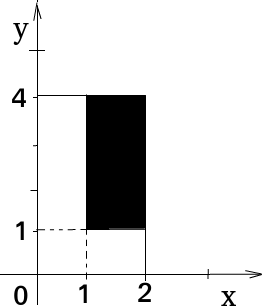
\includegraphics[width=.5\textwidth]{./pictures/4_20.png}
  \caption{Пространство элементарных событий $ \Omega $ и событие $A$}
  \label{fig:420}
\end{figure}

Для того,
чтобы монета не пересекла ни одной из сторон паркета необходимо и достаточно выполнения условий
$1 \leq x \leq 2, \, 1 \leq y \leq 4$, т.е. $A = \left\{ \left( x, y \right): \, 1 \leq x \leq 2, \, 1 \leq y \leq 4 \right\} $.

Имеем
$$P \left\{ A \right\} =
\frac{S_A}{S_{ \Omega }} =
\frac{1 \cdot 3}{2 \cdot 4} =
\frac{3}{8}.$$

\subsubsection*{4.21}

\textit{Задание.} На окружности радиуса $r$ наугад выбраны две точки.
Найдите вероятность того, что расстояние между ними не превышает $r$.

\textit{Решение.} На окружности наугад выбраны две точки $A$ и $B$.
Окружность симметрична, поэтому можем выбрать начало отсчёта в точке $A$.
Обозначим через $x$ длину дуги от начала отсчёта к точке $B$.
Тогда пространство элементарных событий можно описать следующим образом:
$ \Omega =
\left\{ x \in \left[ 0, 2 \pi r \right] \right\} $.
Изобразив $ \Omega $ на прямой, можно убедиться, что $ \Omega $ является отрезком длины $l_{ \Omega } = 2 \pi r$.

Событие $A = $ \{расстояние между точками не превышает $r$\} описывается множеством $A = \left\{ x \leq r \right\} $.
Изобразив $A$ на прямой, можно убедиться, что точки множества $A$ образуют отрезок длиной $l_A = r$.

Тогда вероятность события $A$ равна
$$P \left( A \right) =
\frac{l_A}{l_{ \Omega }} =
\frac{r}{2 \pi r} =
\frac{1}{2 \pi}.$$

\subsubsection*{4.22}

\textit{Задание.} Подсчитайте количество путей:
\begin{enumerate}[label=\alph*)]
\item из $ \left( 0, 0 \right) $ в $ \left( 2n, 0 \right) $ таких, что:
\begin{enumerate}[label=(\roman*)]
\item $S_1 > 0, \dotsc, S_{2n-1} > 0$;
\item $S_1 \geq 0, \dotsc, S_{2n-1} \geq 0$;
\end{enumerate}

\item из $ \left( 0, m \right) $ в $ \left( n, 0 \right) $, таких, что:
\begin{enumerate}[label=(\roman*)]
\item $S_1 > 0, \dotsc, S_{2n-1} > 0$;
\item $S_1 \geq 0, \dotsc, S_{2n-1} \geq 0$.
\end{enumerate}
\end{enumerate}

\textit{Решение.} Путём $ \left\{ S_1, \dotsc, S_x \right\} $ из начала координат в точку
$ \left( x, y \right), \, x \in \\ \in \mathbb{N}, \, y \in \mathbb{N} $
называется ломаная с вершинами в точках
$ \left( 0, 0 \right), \, \left( 1, S_1 \right), \\ \left( 2, S_2 \right), \dotsc, \left( x, S_x \right) $, где $S_x = y, \, S_i - S_{i-1} \in \left\{ -1, 1 \right\} .$

\begin{enumerate}[label=\alph*)]
\item Сведём задачу к задаче, которая решается с помощью метода отражений.
Введём новую систему координат, которая повёрнута относительно данной на $45 \degree $ по часовой стрелке.
В этой системе координат за 1 шаг будет изменяться две координаты (рис. \ref{fig:422}).

\begin{figure}[h!]
  \centering
  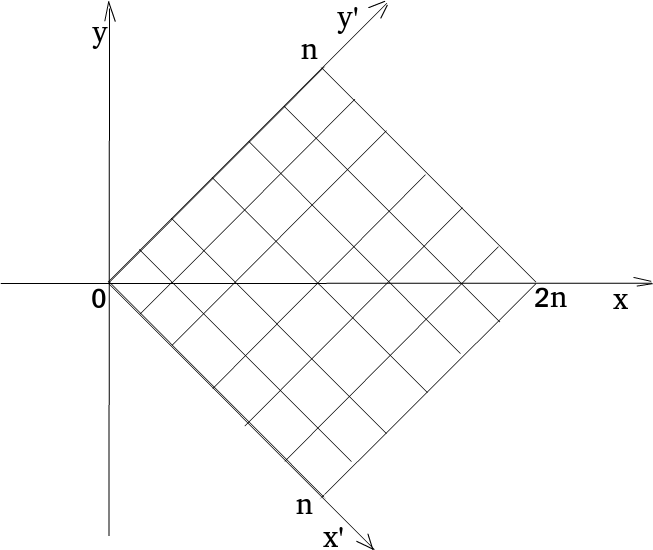
\includegraphics[width=.7\textwidth]{./pictures/4_22.png}
  \caption{Новая система координат}
  \label{fig:422}
\end{figure}

Свели данную задачу к задаче $1.22$.
Имеем пути, состоящие из $n + n$ ходов, среди которых ровно $n$ ходов в направлении $x'$, и $n$ ходов в направлении $y'$.
Если выберем, на каких шагах увеличиваем первую координату, будем знать, где увеличиваем вторую координату.
Это будет $C_{2n}^n$.

\begin{enumerate}[label=(\roman*)]
\item Развернём для удобства рисунок (рис. \ref{fig:4221}).

\begin{figure}[h!]
  \centering
  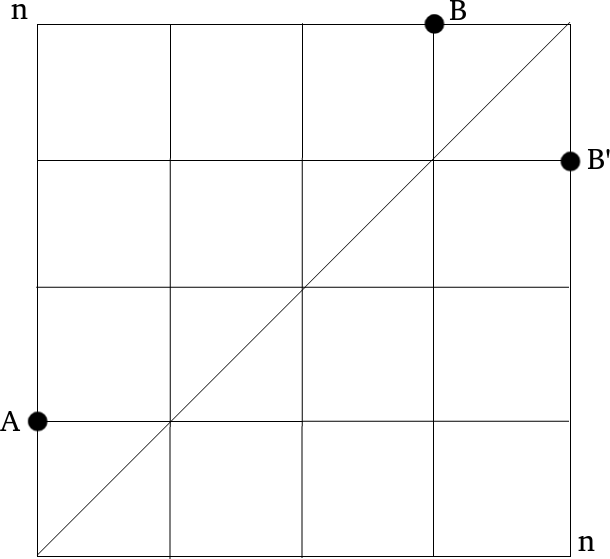
\includegraphics[width=.6\textwidth]{./pictures/4_22_1.png}
  \caption{Метод отражений}
  \label{fig:4221}
\end{figure}

Нам нужно, чтобы путь не касался диагонали,
поэтому уйдём с неё на шаг вверх в точку $A$ и будем искать количество путей из $A$ в $B$.

Количество путей из $A$ в $B$, не цепляющих диагональ,
равно общему количеству путей из $A$ в $B -$ количество путей из $A$ в $B'$.

В точку $A$ из начала координат можно попасть одним способом,
как и в конечную точку из $B$, поэтому количество путей не измениться, если начать считать с них.

Из точки $A$ в точку $B$ есть $n - 1$ вертикальный шаг и $n - 1$ горизонтальный.
Поэтому количество путей из $A$ в $B$ равно $C_{2 \left( n-1 \right)}^{n-1} = C_{2n-2}^{n-1}$.
От этого количества нужно отнять число путей,
которые пересекают диагональ (по условию задачи это те пути, у которых $S_i \leq 0$).
Когда из точки $A$ попадаем на диагональ, есть путь, симметричный данному, который ведёт в точку $B'$.
Есть $n$ горизонтальных шагов и $n - 2$ вертикальных.
Имеем $C_{n+n-2}^n = C_{2n-2}^n$ путей.

Тогда число путей из точки $ \left( 0, 0 \right) $ в точку $ \left( 2n, 0 \right) $ равно
\begin{equation*}
\begin{split}
C_{2n-2}^{n-1} - C_{2n-2}^n =
\frac{ \left( 2n-2 \right)!}{ \left( n-1 \right)! \left( 2n-2-n+1 \right)!} -
\frac{ \left( 2n-2 \right)!}{n! \left( 2n-2-n \right)!} = \\
= \frac{ \left( 2n-2 \right)!}{ \left( n-1 \right)! \left( n-1 \right)!} -
\frac{ \left( 2n-2 \right)!}{n! \left( n-2 \right)!} = \\
= \left( 2n-2 \right)!
\left( \frac{1}{ \left( n-2 \right)! \left( n-1 \right) \left( n-1 \right)! } -
\frac{1}{ \left( n-1 \right)! n \left( n-2 \right)!} \right) = \\
= \left( 2n-2 \right) \cdot \frac{n - n + 1}{\left( n-2 \right)! \left( n-1 \right)! \left( n-1 \right) n} =
\frac{2n-2}{n! \left( n-1 \right)!}.
\end{split}
\end{equation*}

\item Данная задача аналогична предыдущей, только теперь нужно из числа путей из точки с координатами
$ \left( 0, 0 \right) $ в точку с координатами $ \left( 2n, 0 \right) $ отнять число путей, ведущих из точки $ \left( 0, 0 \right) $ в $B'$.

Из точки $ \left( 0, 0 \right) $ в точку $ \left( 2n, 0 \right) $ нужно сделать $n$ горизонтальный шаг и $n$ вертикальных --- всего $C_{2n}^{n}$.

Из точки $ \left( 0, 0 \right) $ в точку $B'$ есть $n$ горизонтальных шагов и $n - 1$ вертикальный.
Всего таких путей $C_{2n-1}^n$.

Итого имеем
\begin{equation*}
\begin{split}
C_{2n}^n - C_{2n-1}^n =
\frac{ \left( 2n \right)!}{n! n!} - \frac{ \left( 2n-1 \right)!}{n! \left( n-1 \right)!} =
\frac{ \left( 2n \right)!}{n! \left( n-1 \right)! n} - \frac{ \left( 2n-1 \right)!}{n! \left( n-1 \right)!} = \\
= \frac{ \left( 2n \right)! - \left( 2n-1 \right)! n}{n! n!} =
\frac{ \left( 2n-1 \right)! \left( 2n-n \right)}{n! n!} =
\frac{ \left( 2n-1 \right)! n}{n! n!};
\end{split}
\end{equation*}
\end{enumerate}

\item задача проиллюстрирована на рисунке \ref{fig:4222}.

\begin{figure}[h!]
  \centering
  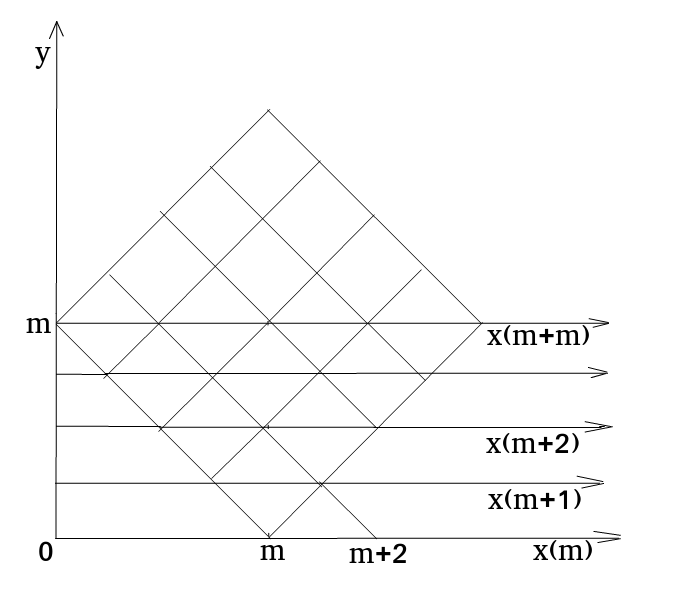
\includegraphics[width=.6\textwidth]{./pictures/4_22_2.png}
  \caption{Пути из точки $ \left( 0, m \right) $ в точку $ \left( n, 0 \right) $}
  \label{fig:4222}
\end{figure}

При $n = m$
существует один путь из точки
$ \left( 0, m \right) $
в точку
$ \left( n, 0 \right)$,
который соответствует линии,
проведённой между этими точками:
$ \left( 0, m \right) \rightarrow \\
\rightarrow \left( 1, m-1 \right) \rightarrow
\left( 2, m-2 \right) \rightarrow \dotsc \rightarrow \left( n, 0 \right)$.

При $n < m$ пути между точками с заданными условиями нет.

При $n > m$ путь возможен только при условии, что $ \left( m-n \right) mod 2 = \\ = 1$.
В каждую следующую точку, в которой выполняется это условие, существует больше путей чем в предыдущую.
Аналогично пункту а) имеем

\begin{enumerate}[label=(\roman*)]
\item
\begin{equation*}
\begin{split}
C_{m+n-2}^{n-1} - C_{m+n-2}^n =
\frac{ \left( m+n-2 \right)!}{ \left( n-1 \right)! \left( m-1 \right)!} -
\frac{ \left( m+n-2 \right)!}{n! \left( m-2 \right)!} = \\
= \frac{ \left( m+n-2 \right)!}{ \left( n-1 \right)! \left( m-2 \right)! \left( m-1 \right)} -
\frac{ \left( m+n-2 \right)!}{ \left( n-1 \right)!n \left( m-2 \right)!}= \\
= \frac{ \left( m+n-2 \right)! \left( n-m+1 \right) }{\left( n-1 \right)! \left( m-2 \right)! \left( m-1 \right) n} =
\frac{ \left( m+n-2 \right)! \left( n-m+1 \right) }{n! \left( m-1 \right)!};
\end{split}
\end{equation*}
\item 
\begin{equation*}
\begin{split}
C_{m+n}^m - C_{m+n-1}^m =
\frac{ \left( m+n \right)!}{m! n!} - \frac{ \left( m+n-1 \right)!}{m! \left( n-1 \right)!} = \\
= \frac{ \left( m+n \right)! - \left( m+n-1 \right)!n}{m!n!} =
\frac{ \left( m+n-1 \right)! \left( m+n-n \right) }{m!n!} = \\
= \frac{ \left( m+n-1 \right)! m}{m!n!}.
\end{split}
\end{equation*}
\end{enumerate}

\paragraph*{Второй способ}

Изобразим путь, который необходимо пройти в декартовых координатах (рис. \ref{fig:4223}).

\begin{figure}[h!]
  \centering
  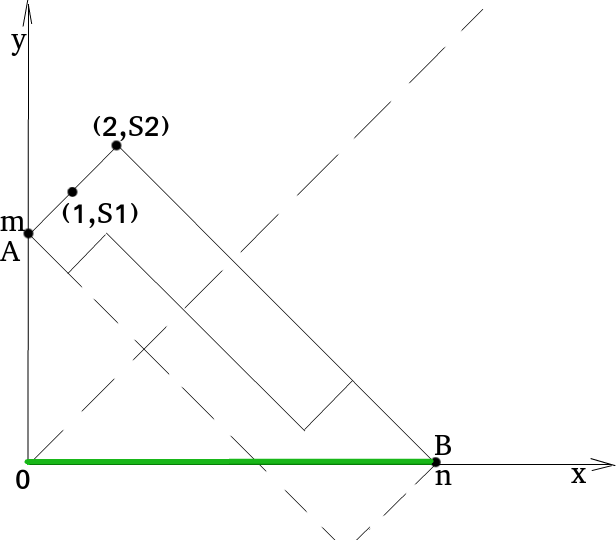
\includegraphics[width=.6\textwidth]{./pictures/4_22_3.png}
  \caption{Путь в декартовых координатах}
  \label{fig:4223}
\end{figure}

Повернём рисунок (рис. \ref{fig:4224}).

\begin{figure}[h!]
  \centering
  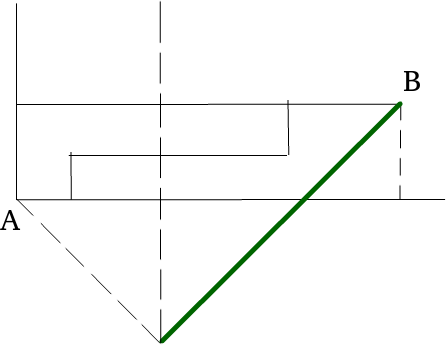
\includegraphics[width=.6\textwidth]{./pictures/4_22_4.png}
  \caption{Путь, который нужно пройти}
  \label{fig:4224}
\end{figure}

Пунктиром обозначены крайние пути, которыми можно пройтись.
Зелёным --- линия, которую нельзя пересекать.
Разница суммы шагов вниз от суммы шагов вверх будет $m$.
Для рисунка \ref{fig:4223} $AB = \sqrt{m^2 + n^2}$ --- гипотенуза треугольника $AOB$.

Самый простой случай: $m = n$ (рис. \ref{fig:4225}).

\begin{figure}[h!]
  \centering
  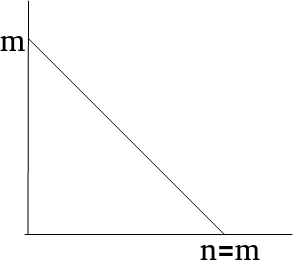
\includegraphics[width=.6\textwidth]{./pictures/4_22_5.png}
  \caption{Случай, когда $m = n$}
  \label{fig:4225}
\end{figure}

Если развернуть, получим прямоугольник шириной $m = n$ и высотой $0$.

Теперь делаем $n = m + 1$.
Высота прямоугольника $1$.
Ширина его $m + 1$.
Задача не решаема, потому что точка $n$ может быть либо под, либо над осью.
Если она под, то до неё не добраться без пересечения оси.
Если над, то она будет не на оси.

Идём дальше: $n = m + 2$.

\begin{figure}[h!]
  \centering
  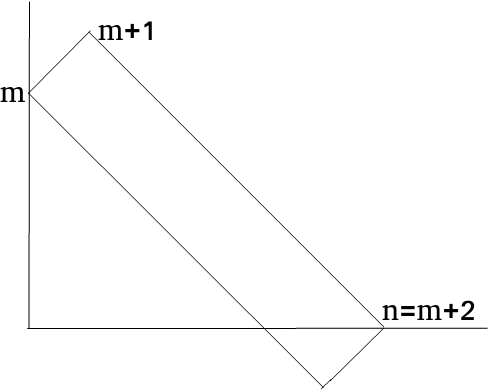
\includegraphics[width=.6\textwidth]{./pictures/4_22_6.png}
  \caption{Случай, когда $n = m + 2$}
  \label{fig:4226}
\end{figure}

Теперь $n$ на оси, форма прямоугольника не поменялась.
И т.д.
Увеличиваем $n$ на $1$ --- получаем прирост высоты и ширины на $1$, увеличиваем $n$ ещё на $1$ --- задача решаема.
Расстояние от $m$ до нижнего угла такое же, как от верхнего угла до точки $n$.
Поскольку с ростом $n$ на $2$ увеличивается $m$ на $1$, а ширина прямоугольника равна высоте этого наклонённого отрезка, то получается, что ширина результирующего прямоугольника растёт на $1$.

Проводим дополнительную вертикальную ось через $m + 2$ (рис. \ref{fig:4227}).

\begin{figure}[h!]
  \centering
  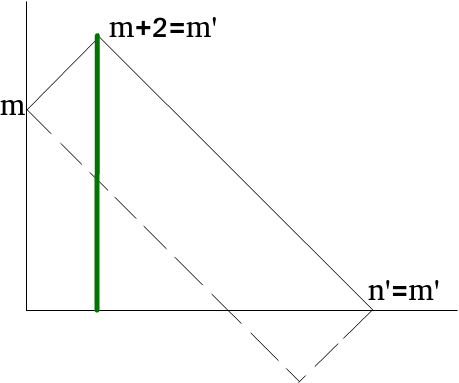
\includegraphics[width=.6\textwidth]{./pictures/4_22_7.png}
  \caption{Дополнительные построения}
  \label{fig:4227}
\end{figure}

Смотрим на верхнюю линию от $m'$ до $n'$.
Это линия длиной $m' = m + 2$.
Значит, весь предыдущий прямоугольник имеет ширину $m + 2$.
Высота 2 --- потому что двух шагов достаточно, чтобы пройтись от $m$ до $m'$.

\begin{figure}[h!]
  \centering
  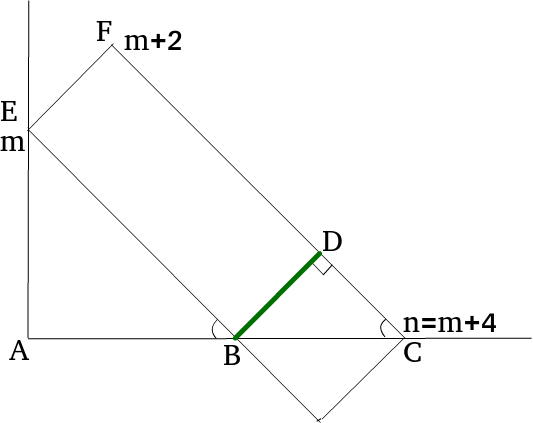
\includegraphics[width=.6\textwidth]{./pictures/4_22_8.png}
  \caption{Дополнительные построения}
  \label{fig:4228}
\end{figure}

Известно, что $AB = m, \, BC = n - m$ (рис. \ref{fig:4228}).
Угол $BCD = 45 \degree$ (можем всегда ходить направо.
При этом либо вниз, либо вверх.
Пройтись направо --- $45 \degree$).
Считаем синус:
$$ \sin \angle BCD =
\cos 45 \degree =
\frac{ \sqrt{2} }{2}.$$
Вычисляем длину $BD$ --- это катет и высота прямоугольника:
$$BD =
BC \cdot \sin \angle BCD =
\left( n-m \right) \cdot \frac{ \sqrt{2} }{2}.$$
Знаем высоту, делим её на $ \sqrt{2} $ --- получаем высоту в шагах:
$$h =
\frac{BD}{ \sqrt{2} } =
\frac{ \left( n-m \right) \sqrt{2} }{2 \sqrt{2} } =
\frac{n-m}{2}.$$

Найдём длину прямоугольника. Она состоит из отрезков $DF$ и $CD$.
$DF = BE$, поэтому найдём его длину из треугольника $ABE$:
$$BE =
\frac{AB}{ \cos \angle ABE} =
\frac{2m}{ \sqrt{2} }.$$
Найдём $CD$ из треугольника $BDC$:
$$CD =
DC \cdot \cos 45 \degree =
\left( n-m \right) \cdot \frac{ \sqrt{2} }{2}.$$
Тогда общая длина равна
\begin{equation*}
\begin{split}
CF =
BE + CD =
\frac{2m}{ \sqrt{2} } + \frac{ \left( n-m \right) \sqrt{2} }{2} =
\frac{2 \sqrt{2} m + \sqrt{2} \left( n-m \right) }{2} = \\
= \frac{ \sqrt{2} \left( 2m+n-m \right) }{2} =
\frac{ \sqrt{2} \left( n+m \right) }{2}.
\end{split}
\end{equation*}

Длина перевёрнутого прямоугольника равна
$$l =
\frac{CF}{ \sqrt{2} } =
\frac{ \sqrt{2} \left( n+m \right) }{2 \sqrt{2} } =
\frac{n+m}{2}.$$

Всего путей из $A$ в $B$ есть
\begin{equation*}
\begin{split}
C_{ \frac{n-m}{2} + \frac{n+m}{2} }^{ \frac{n-m}{2} } =
C_{ \frac{n-m+n+m}{2} }^{ \frac{n-m}{2} } =
C_n^{ \frac{n-m}{2} } =
\frac{n!}{ \left( \frac{n-m}{2} \right)! \left( n - \frac{n-m}{2} \right)! } = \\
= \frac{n!}{ \left( \frac{n-m}{2} \right)! \left( \frac{2n+m-n}{2} \right)!} =
\frac{n!}{ \left( \frac{n-m}{2} \right)! \left( \frac{n+m}{2} \right)!}. 
\end{split}
\end{equation*}

\begin{figure}[h!]
  \centering
  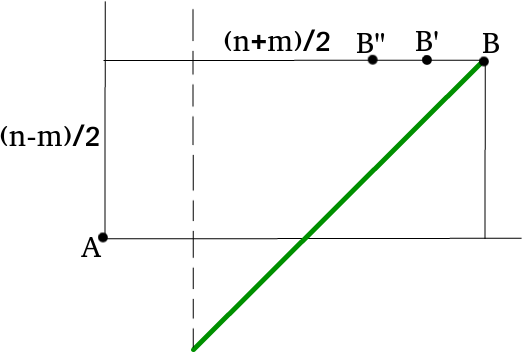
\includegraphics[width=.6\textwidth]{./pictures/4_22_9.png}
  \caption{Вспомогательный рисунок для определения количества путей}
  \label{fig:4229}
\end{figure}

\begin{enumerate}[label=(\roman*)]
\item Посчитаем количество путей, которые не касаются диагонали.
Рассмотрим частный случай.
Пусть $h = 2$ и $l = 4$.
Тогда имеем
$$C_{4+2}^2 =
C_6^2 =
\frac{6!}{2! 4!} =
\frac{5 \cdot 6}{2} =
15$$
возможных путей (рис. \ref{fig:42210}).

\begin{figure}[h!]
  \centering
  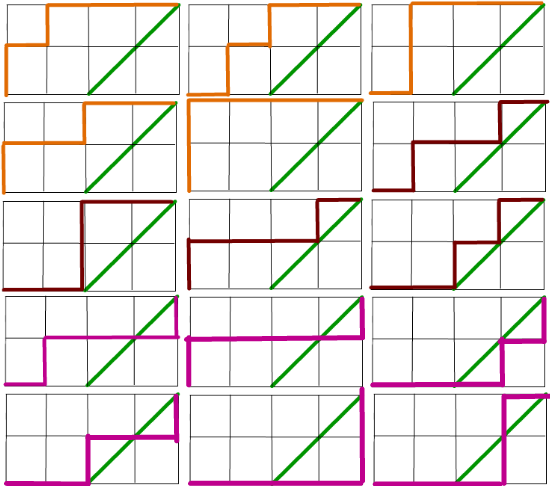
\includegraphics[width=.8\textwidth]{./pictures/4_22_10.png}
  \caption{Все возможные пути для $h = 2$ и $l = 4$}
  \label{fig:42210}
\end{figure}

Оранжевым обозначены пути, которые не касаются диагонали, коричневым --- которые только касаются диагонали, и розовым --- которые пересекают её.
Путей, которые касаются диагонали 10 --- это $C_5^2$.
Т.е. это количество путей из точки $A$ в точку $B'$.
Их
\begin{equation*}
\begin{split}
C_{ \frac{n+m}{2} + \frac{n-m}{2} - 1}^{ \frac{n-m}{2} } =
C_{ \frac{n+m+n-m-2}{2} }^{ \frac{n-m}{2} } =
C_{n-1}^{ \frac{n-m}{2} } = \\
= \frac{ \left( n-1 \right)!}{ \left( \frac{n-m}{2} \right)! \left( n - 1 - \frac{n-m}{2} \right)!} =
\frac{ \left( n-1 \right)!}{ \left( \frac{n-m}{2} \right)! \left( \frac{2n-2-n+m}{2} \right)!} =
\frac{ \left( n-1 \right)!}{ \left( \frac{n-m}{2} \right)! \left( \frac{n+m-2}{2} \right)!} = \\
= \frac{ \left( n-1 \right)!}{ \left( \frac{n-m}{2} \right)! \left( \frac{n+m}{2} - 1 \right)!}.
\end{split}
\end{equation*}

Вероятность равна
\begin{equation*}
\begin{split}
P =
\frac{\frac{ \left( n-1 \right)!}{ \left( \frac{n-m}{2} \right)! \left( \frac{n+m}{2} - 1 \right)!}}{\frac{n!}{ \left( \frac{n-m}{2} \right)! \left( \frac{n+m}{2} \right)!}} =
\frac{ \left( n-1 \right)!}{ \left( \frac{n-m}{2} \right)! \left( \frac{n+m}{2} - 1 \right)!} \cdot
\frac{ \left( \frac{n-m}{2} \right)! \left( \frac{n+m}{2} \right)!}{n!} = \\
= \frac{ \left( n-1 \right)!}{ \left( \frac{n+m}{2} - 1 \right)! } \cdot
\frac{ \left( \frac{n+m}{2} - 1 \right)! \cdot \frac{n+m}{2} }{ \left( n-1 \right)! n} =
\frac{n+m}{2n};
\end{split}
\end{equation*}

\item путей, которые пересекают диагональ 6 или это все пути от $A$ до $B''$, т.е.
\begin{equation*}
\begin{split}
C_{ \frac{n-m}{2} + \frac{n-m}{2} }^{ \frac{n-m}{2} } =
C_{n-m}^{ \frac{n-m}{2} } =
\frac{ \left( n-m \right)!}{ \left( \frac{n-m}{2} \right)! \left( \frac{n-m}{2} \right)! }.
\end{split}
\end{equation*}

Тогда вероятность равна
\begin{equation*}
\begin{split}
P =
\frac{\frac{ \left( n-m \right)!}{ \left( \frac{n-m}{2} \right)! \left( \frac{n-m}{2} \right)! }}{\frac{n!}{ \left( \frac{n-m}{2} \right)! \left( \frac{n+m}{2} \right)!}} =
\frac{ \left( n-m \right)!}{ \left( \frac{n-m}{2} \right)! \left( \frac{n-m}{2} \right)! } \cdot
\frac{ \left( \frac{n-m}{2} \right)! \left( \frac{n+m}{2} \right)!}{n!} = \\
= \frac{ \left( n-m \right)!}{n!} \left( \frac{n+m}{2} \right)! \left( \frac{2}{n-m} \right)!.
\end{split}
\end{equation*}
\end{enumerate}
\end{enumerate}

\subsubsection*{4.23}

\textit{Задание.} В последний тур выборов вышли кандидаты $A$ и $B$.
Кандидат $A$ набрал $n$ голосов, кандидат $B$ --- $m$ голосов.
Избиратели голосовали последовательно.
Найдите вероятность того, что кандидат $A$ не отстал от $B$, если:
\begin{enumerate}[label=\alph*)]
\item $n \geq m$;
\item $n = m$.
\end{enumerate}
 
\textit{Решение.} Вероятность равна
$$P =
\frac{k}{| \Omega |}.$$
Общее количество путей равно $| \Omega| = C_{m+n}^m$.
Найдём $k$.

\begin{enumerate}[label=\alph*)]
\item Данная задача решена в пункте б) из предыдущей.
Так как кандидат $A$ может быть или наравне с кандидатом $B$, или лидировать, то нам подходит пункт ii).
Имеем:
\begin{equation*}
\begin{split}
C_{m+n}^m - C_{m+n-1}^m =
\frac{ \left( m+n \right)!}{m! n!} - \frac{ \left( m+n-1 \right)!}{m! \left( n-1 \right)!} = \\
= \frac{ \left( m+n \right)! - \left( m+n-1 \right)!n}{m!n!} =
\frac{ \left( m+n-1 \right)! \left( m+n-n \right) }{m!n!} = \\
= \frac{ \left( m+n-1 \right)! m}{m!n!}.
\end{split}
\end{equation*}

Тогда вероятность указанного события равна
$$P =
\frac{\frac{ \left( m+n-1 \right)! m}{m!n!}}{C_{m+n}^m} =
\frac{ \left( m+n-1 \right)! m}{m!n!} \cdot \frac{m!n!}{ \left( m+n \right)!} =
\frac{m}{m+n};$$

\item в данном случае $k = 1$.
Поэтому вероятность равна
$$P =
\frac{1}{C_{m+n}^m} =
\frac{m!n!}{ \left( m+n \right)!}.$$
\end{enumerate}

\subsubsection*{4.24}

\textit{Задание.} Решите задачу 4.12 при условии, что в начале работы в кассе буфета было $p$ монет по $50$ коп.

В буфете продаются пирожки стоимостью $50$ коп.
Около буфета собралось $m+n$ студентов,
причём $n$ из них имеют монеты по $50$ коп., а остальные $m$ имеют только по одной гривне $ \left( m \leq n \right) $.
Найдите вероятность того, что ни одном студенту не придётся ждать сдачи,
если в начале работы в кассе было $p$ монет по $50$ коп. 

\textit{Решение.} Данная задача решается методом отражений (рис. \ref{fig:423}).

\begin{figure}[h!]
  \centering
  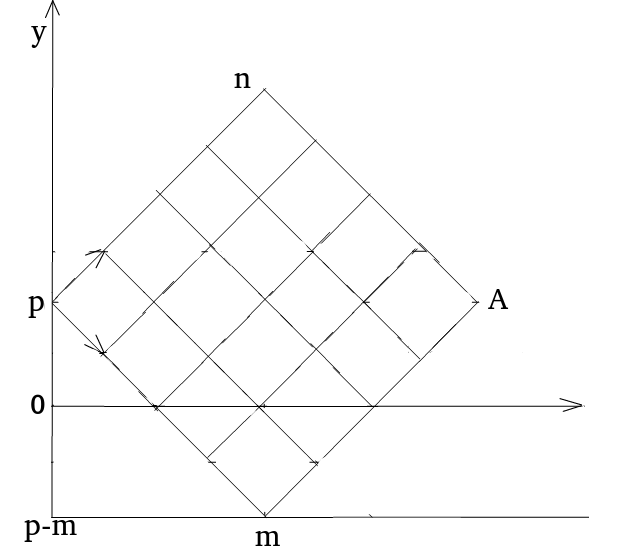
\includegraphics[width=.6\textwidth]{./pictures/4_23.png}
  \caption{Возможные исходы}
  \label{fig:423}
\end{figure}

Точка $ \left( 0, p \right) $ --- начальная, $A$ --- конечная.
Из неё можем двигаться вправо и вверх (если студент заплатил $50$ коп.) или вправо и вниз (если гривну).
Когда студент платит $50$ коп., количество монет в кассе увеличивается на единицу (становится $p + 1$).
Когда студент платит гривну, количество монет в кассе уменьшается на единицу, так как ему необходимо дать сдачу.
Их становится $p - 1$.
Всего есть $C_{n+m}^n$ путей.

Чтобы студент не ждал сдачу, монет в кассе не может быть отрицательное количество, но может быть 0.
Поэтому все пути могут касаться оси, но не пересекать её.
Таких путей 
\begin{equation*}
\begin{split}
C_{p+m}^p - C_{p+m-1}^p =
\frac{ \left( p+m \right)!}{p!m!} - \frac{ \left( p+m-1 \right)!}{p! \left( m-1 \right)!} = \\
= \frac{ \left( p+m \right)!}{p! \left( m-1 \right)! m} - \frac{ \left( p+m-1 \right)!}{p! \left( m-1 \right)!} =
\frac{ \left( p+m-1 \right)!m}{p!m!}.
\end{split}
\end{equation*}
